% Autor: Simon May
% Datum: 2014-08-12
\section{Münsterrätsel}
Im Folgenden seht ihr fünf Verkehrsschilder aus Münster. Wer von euch es als Erster schafft, bis zum 31.~Oktober 4 von 5 Schildern an ihrem Platz zu fotografieren, bekommt einen Preis. Dieser kann im Fachschaftsraum abgeholt werden.

\vspace{0cm plus 1cm}
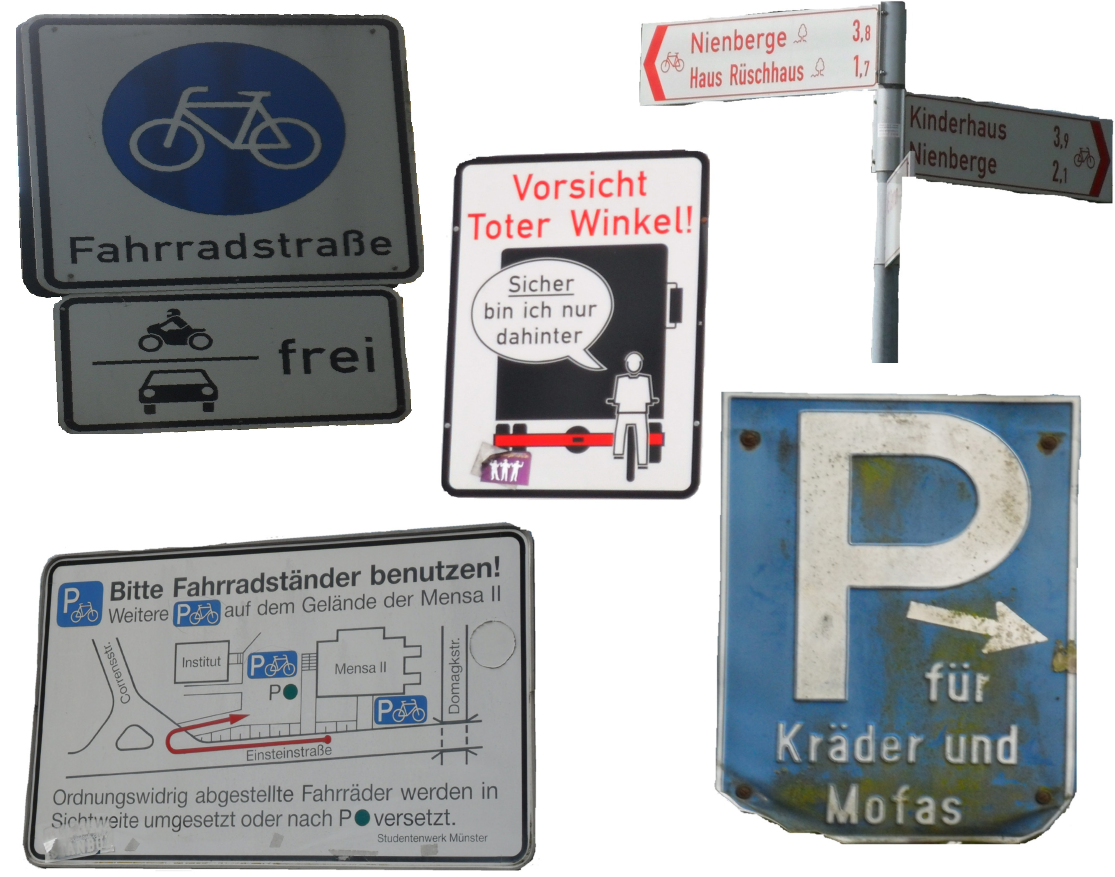
\includegraphics[width=\textwidth]{res/muensterraetsel_schilder.pdf}

\section*{Fortsetzung Münsterrätsel}
In diesem Rätsel findet ihr waagerecht, senkrecht und diagonal die wichtigsten Kneipen und Discos in Münster, die ihr kennen sollten. Viel Spaß beim Suchen!

\begin{center}
\includegraphics[width=0.92\textwidth]{res/muensterraetsel_kreuzwort.jpg}

\includegraphics[width=0.6\textwidth]{res/comics/darts.jpg}
\rotatebox{90}{\tiny\url{http://www.dartsport-rostock.de/dartsport_rostock_lustiges.html}}
\end{center}

\subsection*{Überlebenstraining für Physiker in Münster}
\begin{multicols}{2}
\textbf{Die Antworten auf die folgenden Fragen könnten für euch im Verlaufe eures Studiums absolut lebensnotwendig werden\dots\ oder auch nicht!}

\begin{enumerate}[font=\large, before=\large]
\item Wie wird Münsters erste akademische Bieranstalt genannt?
	\begin{enumerate}[label=\alph*), before=\normalsize]
	\item Destille
	\item Cavete
	\item Das Blaue Haus
	\item Pinkus Müller
	\end{enumerate}
\item Welche chemische Verbindung sorgt dafür, dass man am Aasee-Ufer ohne Atemschutzmaske joggen/grillen kann?
	\begin{enumerate}[label=\alph*), before=\normalsize]
	\item Fe(II)Cl
	\item Fe(III)Cl
	\item C\textsubscript{2}H\textsubscript{5}OH
	\item H\textsubscript{1}N\textsubscript{1}
	\end{enumerate}
\item Welche Wochentage gehen auf Namen germanischer Götter zurück?
	\begin{enumerate}[label=\alph*), before=\normalsize]
	\item Dienstag, Donnerstag, Freitag
	\item Dienstag, Mittwoch, Donnerstag
	\item Donnerstag, Freitag, Samstag
	\item Alle
	\end{enumerate}
\item "$\Xi$" -- Hä, Was ist denn das?
	\begin{enumerate}[label=\alph*), before=\normalsize]
	\item Xi
	\item Psi
	\item Chi
	\item Omikron
	\end{enumerate}
\item Wie heißt das Gebilde vor der Physik-Fachschaft?
	\begin{enumerate}[label=\alph*), before=\normalsize]
	\item Quadratische Senkung
	\item Hässliches Betonloch
	\item Mahnmal zur Vergänglichkeit des Menschen im Kontrast zur Beständigkeit des Betons besonders in pyramidaler Darstellung
	\item Heinz
\end{enumerate}
\item Und wer hat es ausgedacht?
	\begin{enumerate}[label=\alph*), before=\normalsize]
	\item Bruce Lee
	\item Bruce Darnell
	\item Bruce Nauman
	\item Bruce "Schweinebacke" Willis
	\end{enumerate}
\item Wie viel kostet ein vegetarischer Mensa-Burger?
	\begin{enumerate}[label=\alph*), before=\normalsize]
	\item \SI{2,20}{\euro}
	\item \SI{1,95}{\euro}
	\item \SI{1,50}{\euro}
	\item igitt
	\end{enumerate}
\item Welche Chemie-Formel kann sich kein Chemiker merken?
	\begin{enumerate}[label=\alph*), before=\normalsize]
	\item $n = \sfrac{m}{M}$
	\item $n M = m$
	\item $\sfrac{1}{n} = \sfrac{M}{m}$
	\item $\sfrac{n M}{m} = 1$
	\end{enumerate}
\item Was kann man im Münsteraner Zoo füttern?
	\begin{enumerate}[label=\alph*), before=\normalsize]
	\item afrikanische Elefanten
	\item indische Elefanten
	\item asiatische Elefanten
	\item deutsche Elefanten
	\end{enumerate}
\end{enumerate}

\hfill(Lösung auf Seite \pageref{rätsel_lösungen})

\begin{center}
\includegraphicscompressed[width=0.7\columnwidth]{res/bart_simpson_andi.png}
\end{center}
\end{multicols}
